\documentclass[12pt,a4paper]{article}
\usepackage[utf8]{inputenc}
\usepackage[T1]{fontenc}
\usepackage{amsmath,amssymb,amsfonts}
\usepackage{hyperref}
\usepackage{geometry}
\usepackage{booktabs}
\usepackage{longtable}
\usepackage{amsthm}
\usepackage{graphicx}
\newtheorem{theorem}{Theorem}
\newtheorem{proposition}[theorem]{Proposition}
\newtheorem{lemma}[theorem]{Lemma}
\newtheorem{corollary}[theorem]{Corollary}
\newtheorem{conjecture}[theorem]{Conjecture}
\theoremstyle{remark}
\newtheorem{remark}[theorem]{Remark}
\geometry{a4paper, margin=1in}
\title{Arithmetic Chaos with Rare Islands of Order:\\
A Computational Map of the Collatz Space\\
\large Part I: The Computational Map}
\author{Collatz Crystal Hunter Project}
\date{August 2026}
\begin{document}
\maketitle
\begin{abstract}
We present a large-scale computational study of Collatz trajectories in terms of
accelerated odd dynamics, shift-vectors, and confluence structures, up to
$\sim310$ bits and trajectory lengths $d\approx500$. The central discovery is
\textbf{Zone~2} --- a family of $913$ numbers (bit lengths $71$--$87$) whose
trajectories merge into a single $75$-bit node
$x^*=20152090995747160937051$ within $\le7$ odd steps and then follow an
identical path to a peak of $140$ bits. In parallel, Barina's number is an
isolated second path to the same peak. A systematic census reveals confluence
centers for all integer peaks $14$--$51$ plus peak $140$ ($39$ centers),
forming a continuous archipelago. We find the scaling law
$\mathrm{bits}(c)=0.498258\cdot\mathrm{peak}+6.2928$ ($R^2=0.965$, primary
centers) and the modular filter $c\equiv2\pmod3$. Cluster analysis separates
\textbf{Class~A} (deep funnels: $121$, $x^*$; $100\%$ hit rate,
$S/d\approx1.33$) from \textbf{Class~B} (shallow confluences, $72$--$93\%$).
A dead zone ($88$--$170$ bits) free of ratio anomalies is confirmed by four
independent methods. The body of results indicates that the Collatz space is a
continuous archipelago of confluence structures (\textbf{Class~B}) above which
rise rare deep funnels (\textbf{Class~A}) organized around $\log_2 3$.
This is Part~I of a two-part programme; the companion Part~II supplies the
large-deviation theory explaining these structures.
\smallskip
\noindent\textit{Companion paper:} \textit{Crystals Cannot Be Grown: A
Large-Deviation Theory of Typical and Rigid Collatz Structures} (Part~II).
\end{abstract}

\section*{Glossary and Constants}
\begin{itemize}
\item \textbf{Family A ($2^b-1$)}: base landscape; ratios $\to\log_2 3\approx1.585$.
\item \textbf{Confluence}: capture of trajectories into nodes (centers).
\item \textbf{Class A (deep funnels)}: $100\%$ hit rate; centers $121$ (peak 14), $x^*$ (peak 140).
\item \textbf{Class B (shallow funnels)}: $72$--$93\%$ hit rate; dense archipelago (peaks 14--51).
\item \textbf{Center-bits formula}: $\mathrm{bits}(c)=0.498258\,\mathrm{peak}+6.2928$ ($R^2=0.965$); refit over all 39 centers $0.620145\,\mathrm{peak}+2.2850$ ($R^2=0.916$).
\item \textbf{Scaling Hypothesis $\times10$}: Class~A centers follow a logarithmic scale ($14\to140\to1400$); constructive routes closed (Part~I \S\ref{sec:dead}); existence open.
\item \textbf{Septembrino's Law}: divisor distribution $P(\mathrm{div}=2^a)=2^{-a}$.
\end{itemize}

\section{Introduction and Chronology}
\subsection{The Collatz problem}
For $n\in\mathbb N$ define $T(n)=n/2$ (even) and $T(n)=(3n+1)/2$ (odd). The
Collatz conjecture states that iterating $T$ from any $n$ reaches $1$. The
anomaly of a number is its \emph{ratio} (peak bits / input bits); typical
numbers give ratio $\approx1.0$--$1.2$; Family~A gives ratio $\to\log_2 3$.
\subsection{Starting point: Barina's records}
Barina's exhaustive search to $2^{71}$ lists two $71$-bit record holders with
peak $140$; these seeded the study.
\subsection{Phases}
\textbf{Phase 1} (Markov search, 35 cores): best ratio $1.613$ for 73--80 bits.
\textbf{Phase 2} (30M records): ratio peak $\approx1.04$; max-ratio$\times$bits
recomputed per bit length always equals $140$ (the ``magnetic peak'').
\textbf{Phase 3} (structural): CRT constructor, shift-vector analyzer, reverse
trees, beam search; all results below obtained.

\section{Notation and Accelerated Dynamics}
We use accelerated odd dynamics
$x_{k+1}=(3x_k+1)/2^{a_k}$ with $a_k\ge1$; the shift-vector is
$(a_0,\dots,a_{d-1})$; $S_k=\sum_{i<k}a_i$; after $k$ steps
$x_k=(3^k x_0+c_k)/2^{S_k}$, $c_0=0$, $c_{k+1}=3c_k+2^{S_k}$.
The cumulative gain is $G(k)=k\log_2 3-S_k$; the peak is near $\max G$.
Every prefix defines a residue class $x_0\equiv r_k\pmod{2^{S_k}}$.
\subsection{2-adic interpretation}
An admissible word $w$ defines a cylinder $C(w)=\rho(w)+2^{S_d}\mathbb Z_2$ of
Haar measure $2^{-S_d}$. \textbf{Zone~2} is a cylinder of measure $2^{-342}$;
$27$ gives $2^{-70}$; Barina gives $2^{-271}$. The archipelago is a finite set
of exceptional cylinders separated by vast regions of exponentially small
growing-path measure, consistent with Tao's almost-all decay.
\begin{remark}[Septembrino's parameterization]
$N=k\cdot3^m-1$ parameterizes the Haar measure in $\mathbb Z_2$; the observed
periodicity of $v_2(N)$ follows from $3^n\bmod2^p$, placing it in classical
$p$-adic dynamics.
\end{remark}

\section{Base Layer: Family A}
Numbers $2^b-1$ have shift-vectors $94$--$97\%$ ones, ratio $\to\log_23$,
$S/d\approx0.99$ --- the landscape level. Full spectral analysis $b=71$--$310$
found $10$ values with $S/d>1.05$ (micro-plateaus at peaks $183,190,280,483,494$),
all resonances of $\log_23$ continued-fraction approximations; verification
showed micro-plateaus exist only for $2^b-1$ itself.

\section{Zone 2: The Only Confirmed Major Confluence Class}
\subsection{Discovery and representatives}
Barina record holders (71--82 bits) all peak at $140$ with shift-vectors
identical from position 8; \textbf{Zone~2} found for all bits $71$--$87$.
\begin{longtable}{lllll}
\toprule
\textbf{Bits} & \textbf{Number $n$} & \textbf{Peak} & \textbf{Ratio} & \textbf{Steps to $x^*$} \\
\midrule
71 & 2358909599867980429759 & 140 & 1.9718 & 7 \\
75 & 37742553597887686876149 & 140 & 1.8667 & 7 \\
80 & 1207761715132405980037043 & 140 & 1.7500 & 7 \\
87 & 154593499536947965444748439 & 140 & 1.6092 & 7 \\
\bottomrule
\caption*{Representatives (full 17-row table in Supplementary). All have $d=259$, $S=\mathrm{bits}+271$.}
\end{longtable}
$2^{88}-1$ peaks at $141$ and does \emph{not} pass through $x^*$ --- the sharp boundary.

\begin{figure}[h]
    \centering
    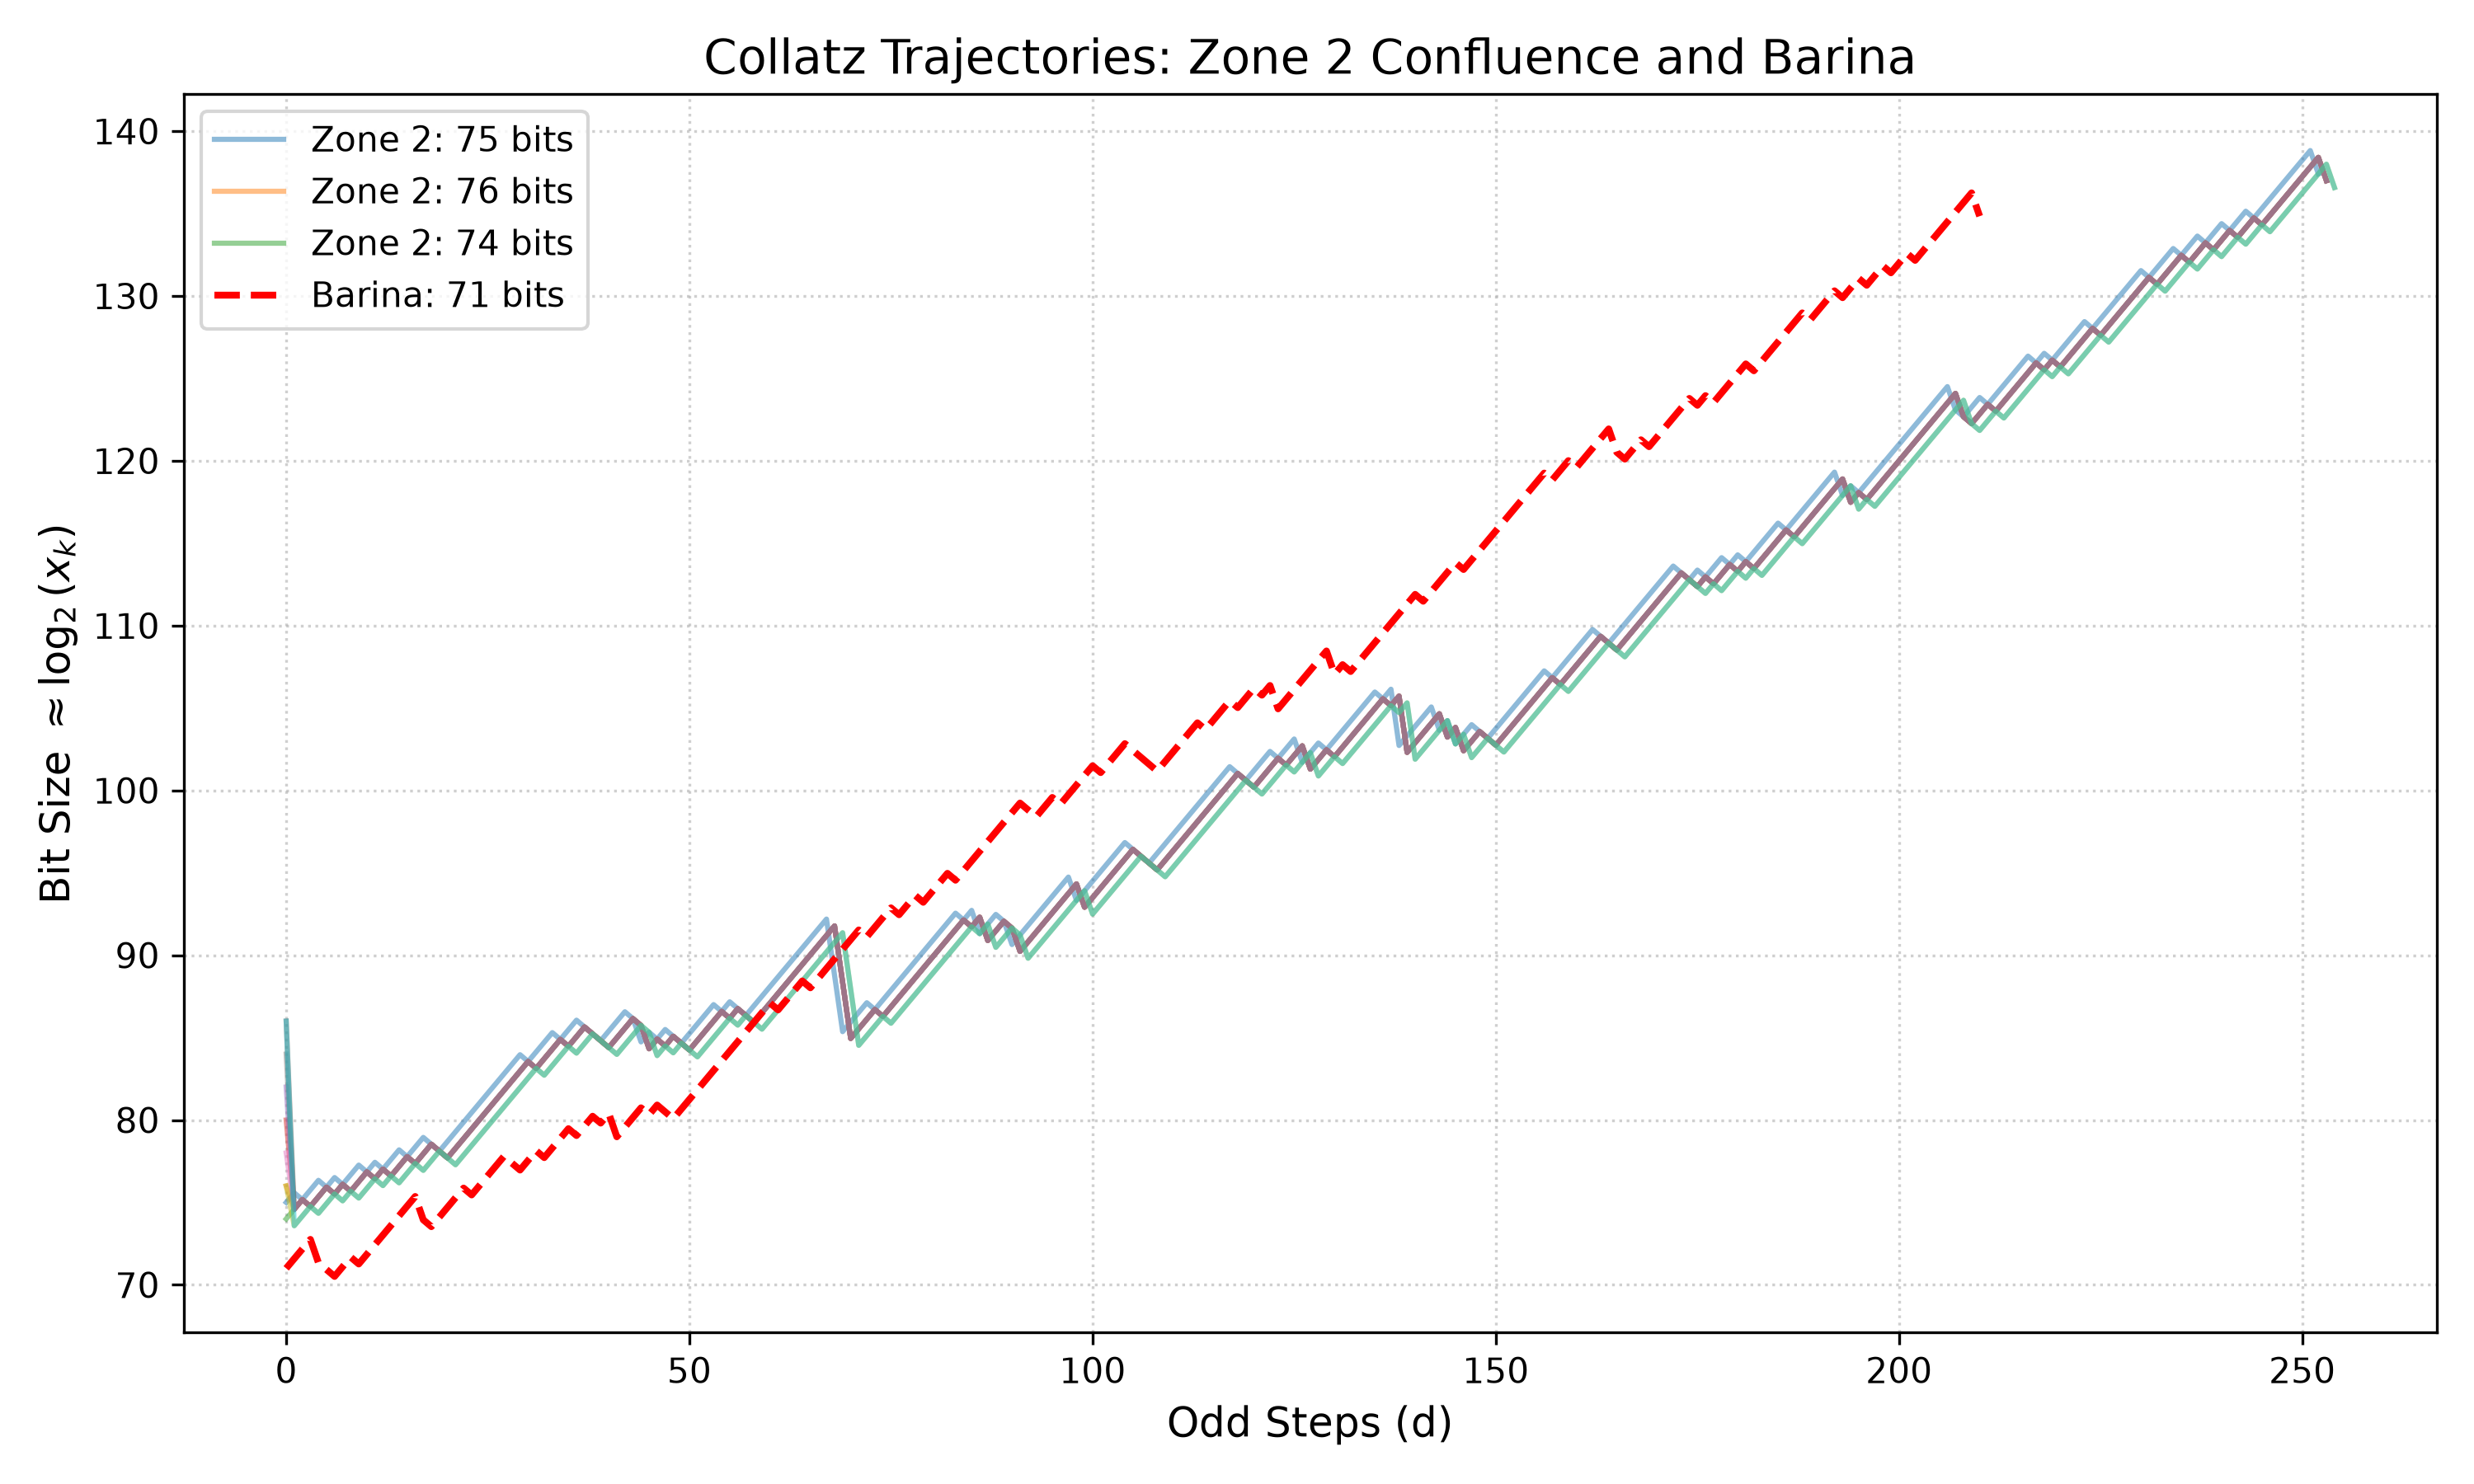
\includegraphics[width=0.8\textwidth]{../data/trajectory_plot.png}
    \caption{Trajectories of Zone 2 numbers (solid) perfectly merging into $x^*$, compared to Barina's number (dashed) reaching the same peak independently.}
    \label{fig:trajectory}
\end{figure}

\subsection{Two-layer invariants}
\textbf{Core} ($x^*\to$ peak): identical for all 913; $d_{core}=251$,
$S_{core}=334$, $S/d\approx1.331$. \textbf{Adapter shell}: inputs reach $x^*$ in
$k\in[0,7]$ steps; outer shell ($k=7$) obeys $S_{adapter}=\mathrm{bits}-63$;
adapter entropy $\approx0.395$ bits$^{-1}$; adapter determined by lowest 19 bits.
\subsection{Confluence point $x^*$}
\begin{theorem}[Computational]
All 17 representatives (bits 71--87, $d=259$) arrive at
$x^*=20152090995747160937051$ (75 bits) in $\le7$ odd steps; trajectories then
identical (exact equality) for 252 steps to peak 140. $2^{88}-1$ does not pass $x^*$.
\end{theorem}
\subsection{Reverse tree and full size}
Reverse tree of $x^*$ to depth 7 (bits $\le90$): 1859 nodes, 913 with bits
71--87; all 913 yield peak 140 (100\%). Inputs double per bit.
\subsection{Grammar and the $(1,1,2)$ equilibrium}
FFT shows periods $T\approx10,6.3,18$; critical tail shows staircase $[2,1,1]$,
the shadow of the $3$-adic point $-29/11$.
\begin{lemma}[$(1,1,2)$ periodic equilibrium]
$R_a(x)=(x2^a-1)/3$; $F=R_2\circ R_1\circ R_1=(16x-29)/27$, a contraction on
$\mathbb Z_2$ ($|16/27|_2=2^{-4}$) with fixed point $\xi=-29/11$; mean shift
$4/3$, gain $\log_23-4/3\approx0.2516$, matching body growth $\sim0.25$.
\end{lemma}
The core satisfies $S/d\approx1.331$ (within $0.2\%$ of $4/3$): the core is the
vacuum $\xi$ dressed by a sparse defect gas. (Full instanton analysis: Part~II.)

\section{Barina's Number: An Isolated Second Path}
$n=1765856170146672440559$ (71 bits, $d=213$, $S/d=1.263$) reaches peak 140 via
a path sharing no intermediate point with Zone~2 (even mod $2^{30}$); common
prefix $[1,1,1]$; reverse tree from Barina's peak empty (peak odd value
$\equiv0\pmod3$, no predecessors). Same peak, two independent mechanisms.

\section{Number 27 as a Miniature Zone 2}
$27$: $d_{peak}=28$, $S/d\approx1.36$, shift profile near-identical to Zone~2;
$x_7=121$ is a confluence center (reverse tree depth 5: 27 inputs, 100\% peak 14);
similarity score $\{x^*,27\}$ vs $\{\text{Barina}\}\approx0.989$.

\section{Dead Zone 88--170 Bits}\label{sec:dead}
No ratio $>1.585$ found in 88--170 bits by four methods (peak hunter, parity
scan $>14$M checks, beam search $\pm$ niching). \textbf{Corollary.} After
Zone~2 (boundary 87 bits) no new confluence \emph{ratio} anomaly to 170 bits.
\subsection{Probabilistic anatomy (Sanov)}
Under the i.i.d.\ shift heuristic, $P(S/d\le1.40)\sim2^{-d\,D_{\rm KL}(q\|p)}$,
$D_{\rm KL}\approx0.28$; for $d>300$, $<10^{-25}$. (A heuristic, not a bound.)
\subsection{Algebraic impossibility of shadow zones (CRT dimensionality)}
\begin{proposition}[CRT dimensionality trap]
An admissible block $w$ of shift $S$ repeated $m$-fold occupies one residue
class mod $2^{mS}$; for target bits $B<mS$ the expected count is $\approx2^{B-mS}$.
\end{proposition}
For Barina ($S\approx269$) a 2-fold echo at $B=142$ has expectation $2^{-396}$;
Zone~2 core ($S=342$--$358$) gives $\le2^{-514}$; $x^*$ gives $\le2^{-496}$.
Constructive CRT lifts confirm echoes exist near $B\approx2S$ (670/544 bits) but
with ratios $1.19$/$1.25<1.585$: algebraically natural echoes fail to breach the
large-deviation limit.
\subsection{Control-budget obstruction}
A defect $a\ge3$ forces a clean run $L\ge(a-\bar a_t)/(\bar a_t-\bar a_p)$;
with $\bar a_p=4/3$, $L_{\min}\approx82.5$--$99\gg L_{\max}\approx3.4$ for $B=4$.
\begin{corollary}[Closure of constructive Scaling $\times10$]
No bounded-branching constructive lifting assembles a Class~A macro-soliton.
\end{corollary}
\begin{remark}[Existence vs.\ constructibility]
The obstruction is algorithmic, not ontological: solitons can be found, not grown.
\end{remark}

\section{Refutation of Zone 3}
Candidates (peaks 237--244, 145--150 bits) are Family~A neighbourhood (density
$1.000$, bit-inversion fragility identical to Family~A). Zone~3 does not exist.

\section{Archipelago of Confluence Centers}
\subsection{Census (peaks 10--200)}
Verification (reverse tree, depth 7) confirmed centers for all integer peaks
14--51 plus 140. Directed search (up to $5.7\times10^9$ candidates/peak) found
centers for every peak 31--50. Recurring hubs (2051, 23) are \emph{descent}
transit hubs, not caustics (filtered out).
\begin{longtable}{lllllll}
\toprule
\textbf{Peak} & \textbf{Center} & \textbf{Bits} & \textbf{Inputs} & \textbf{HR} & $d_{peak}$ & $S/d$ \\
\midrule
14 & 719 & 10 & 33 & 80.5\% & 3 & 1.00 \\
14 & $121$ (A) & 7 & 27 & 100\% & 21 & 1.38 \\
20 & 4763 & 13 & --- & 100\% & --- & --- \\
30 & 58595471 & 26 & 31 & 81.6\% & 3 & 1.00 \\
40 & 35337455 & 26 & 343 & 91.7\% & 41 & 1.27 \\
50 & 1396693151 & 31 & 716 & 88.5\% & 53 & 1.26 \\
51 & 6572463707 & 33 & $\approx400$ & 88.0\% & 56 & 1.29 \\
140 & $x^*$ (A) & 75 & 913 & 100\% & 250 & 1.33 \\
\bottomrule
\caption*{Selected rows; full 39-center table in Supplementary.}
\end{longtable}
\subsection{Two classes; continuum of caustics}
Class~A $\{121,x^*\}$: $100\%$ HR, $S/d\approx1.357$, compact (bits/peak
$\approx0.518$), long path. Class~B: $72$--$92\%$, $S/d\approx1.252$.
Depth-resolved HR shows Class~B/transitional collapse by depth 4--5 while $x^*$
holds $\ge95.9\%$ to depth 9: Class~A is singular; transitional centers are the
strong end of Class~B. Genuine ascending centers reach $HR=1.0$ as the window
deepens (local caustics); transit hubs dissolve ($HR\to0$).
\subsection{Centers do not cover the space}
$156/17000$ ($0.92\%$) random trajectories pass a center; $0/14$ with ratio$>1.5$.

\section{Spectrum of Chords}
$S/d$ is chord strength: Family~A $0.99$; weak $1.05$; intermediate $1.19$;
Zone~2 (Barina) $1.26$; Zone~2 core $1.32$; $27$ at $1.36$ --- a continuous
spectrum, Zone~2 and 27 in the same range.

\section{Summary Map}
Family~A base; continuous Class~B archipelago (peaks 14--51); two Class~A deep
funnels; Zone~2 (913 inputs, $x^*$); Barina isolated; dead zone 88--170;
plateaus 280/483 as Family~A resonances; macro-centers non-constructible
($\Delta\ge2P$).

\section{The Big Picture}
The space is a continuous field of confluence structures (Class~B) above which
rise rare deep funnels (Class~A). Crystals can be found, not grown (triad of
obstructions: Sanov, CRT dimensionality, control budget). Scaling $\times10$ is
a question of existence, not constructibility.

\section{Computational Complexity}
Exhaustive parity scan $\mathcal O(2^{bits})$ (infeasible $>90$); reverse tree
$\mathcal O(B^{depth})$ (Zone~2 in ms); residue beam search (to 170 bits);
confluence census ($22.9\times10^9$ candidates for peak 51).

\section{Open Questions}
Archipelago beyond peak 50; existence of $x^{**}$ (peak 1400); nature of
$\alpha=1/2$; Barina's intermediate point; compatibility with Tao's theorem;
$\mathbb Z_2$-corridor stability of Class~A vs B. (Theoretical explanations of
all the above are developed in Part~II.)

\section*{Data Availability and Supplementary Material}
Full Zone~2 catalog (913 entries), 39-center census, KL derivation, beam-search
death logs, and algorithmic pseudocodes are in the Supplementary Material and
the project GitHub repository (see README). All verification scripts
(\texttt{zone\_parity\_search.py}, \texttt{reverse\_tree\_xstar.py},
\texttt{confluence\_census.py}, \texttt{verify\_census\_centers.py},
\texttt{targeted\_search\_31\_50.py}, \texttt{two\_class\_analysis.py},
\texttt{basin\_test.py}, \texttt{family\_a\_spectrum.py},
\texttt{automaton\_invariants.py}, etc.) are released with the repository.

\section{Conclusion: The Computational Foundation}
This Part has constructed a complete computational map of the Collatz space to
$\sim310$ bits: Zone~2 (913 inputs, two-layer core+adapter), the continuous
archipelago (39 centers, scaling law, two classes), the $(1,1,2)$ vacuum, the
dead zone, and the triad of obstructions closing all constructive routes.
\textbf{Philosophical conclusion.} The space is not ``chaos with rare islands''
but a continuous field of confluence structures above which rise rare deep
funnels; these can be found but not grown. The theoretical explanation --- the
large-deviation duality, dressed-vacuum anatomy, and the two-heads dichotomy ---
is developed in the companion Part~II.

\begin{thebibliography}{99}
\bibitem{Lagarias1985} Lagarias, J.C. (1985). \textit{The 3x+1 problem and its generalizations}. Amer. Math. Monthly 92(1), 3--23.
\bibitem{Tao2022} Tao, T. (2022). \textit{Almost all orbits of the Collatz map attain almost bounded values}. Forum Math. Sigma 10, e12.
\bibitem{Barina2021} Barina, D. (2021). \textit{Convergence verification of the Collatz problem}. J. Supercomputing 77, 2681--2688.
\bibitem{Dembo1998} Dembo, A., Zeitouni, O. (1998). \textit{Large Deviations Techniques and Applications}. Springer.
\bibitem{PartII} Collatz Crystal Hunter Project. \textit{Crystals Cannot Be Grown: A Large-Deviation Theory of Typical and Rigid Collatz Structures} (Part II).
\end{thebibliography}
\end{document}
